%%%%%%%%%%%%%%%%%%%%%%%%%%%%%%%%%%%%%%%%%
% Article EcoFoG
% Version 2.1 (23/10/2017)
%
% adapté de :
% Stylish Article
% LaTeX Template
% Version 1.0 (31/1/13)
%
% This template has been downloaded from:
% http://www.LaTeXTemplates.com
%
% Original author:
% Mathias Legrand (legrand.mathias@gmail.com)
%
% License:
% CC BY-NC-SA 3.0 (http://creativecommons.org/licenses/by-nc-sa/3.0/)
%
%%%%%%%%%%%%%%%%%%%%%%%%%%%%%%%%%%%%%%%%%


%----------------------------------------------------------------------------------------
%	PACKAGES AND OTHER DOCUMENT CONFIGURATIONS
%----------------------------------------------------------------------------------------

\documentclass[fleqn,10pt]{ArtEcoFoG} % Document font size and equations flushed left

\setcounter{tocdepth}{3} % Show only three levels in the table of contents section: sections, subsections and subsubsections


% Pandoc environments
\usepackage{framed}
\usepackage{fancyvrb}
\providecommand{\tightlist}{%
  \setlength{\itemsep}{0pt}\setlength{\parskip}{0pt}}
\newcommand{\VerbBar}{|}
\newcommand{\VERB}{\Verb[commandchars=\\\{\}]}
\DefineVerbatimEnvironment{Highlighting}{Verbatim}{commandchars=\\\{\}, fontsize=\scriptsize} % Code R
\definecolor{shadecolor}{RGB}{248,248,248}
\newenvironment{Shaded}{\begin{snugshade}}{\end{snugshade}}
\newcommand{\KeywordTok}[1]{\textcolor[rgb]{0.13,0.29,0.53}{\textbf{{#1}}}}
\newcommand{\DataTypeTok}[1]{\textcolor[rgb]{0.13,0.29,0.53}{{#1}}}
\newcommand{\DecValTok}[1]{\textcolor[rgb]{0.00,0.00,0.81}{{#1}}}
\newcommand{\BaseNTok}[1]{\textcolor[rgb]{0.00,0.00,0.81}{{#1}}}
\newcommand{\FloatTok}[1]{\textcolor[rgb]{0.00,0.00,0.81}{{#1}}}
\newcommand{\ConstantTok}[1]{\textcolor[rgb]{0.00,0.00,0.00}{{#1}}}
\newcommand{\CharTok}[1]{\textcolor[rgb]{0.31,0.60,0.02}{{#1}}}
\newcommand{\SpecialCharTok}[1]{\textcolor[rgb]{0.00,0.00,0.00}{{#1}}}
\newcommand{\StringTok}[1]{\textcolor[rgb]{0.31,0.60,0.02}{{#1}}}
\newcommand{\VerbatimStringTok}[1]{\textcolor[rgb]{0.31,0.60,0.02}{{#1}}}
\newcommand{\SpecialStringTok}[1]{\textcolor[rgb]{0.31,0.60,0.02}{{#1}}}
\newcommand{\ImportTok}[1]{{#1}}
\newcommand{\CommentTok}[1]{\textcolor[rgb]{0.56,0.35,0.01}{\textit{{#1}}}}
\newcommand{\DocumentationTok}[1]{\textcolor[rgb]{0.56,0.35,0.01}{\textbf{\textit{{#1}}}}}
\newcommand{\AnnotationTok}[1]{\textcolor[rgb]{0.56,0.35,0.01}{\textbf{\textit{{#1}}}}}
\newcommand{\CommentVarTok}[1]{\textcolor[rgb]{0.56,0.35,0.01}{\textbf{\textit{{#1}}}}}
\newcommand{\OtherTok}[1]{\textcolor[rgb]{0.56,0.35,0.01}{{#1}}}
\newcommand{\FunctionTok}[1]{\textcolor[rgb]{0.00,0.00,0.00}{{#1}}}
\newcommand{\VariableTok}[1]{\textcolor[rgb]{0.00,0.00,0.00}{{#1}}}
\newcommand{\ControlFlowTok}[1]{\textcolor[rgb]{0.13,0.29,0.53}{\textbf{{#1}}}}
\newcommand{\OperatorTok}[1]{\textcolor[rgb]{0.81,0.36,0.00}{\textbf{{#1}}}}
\newcommand{\BuiltInTok}[1]{{#1}}
\newcommand{\ExtensionTok}[1]{{#1}}
\newcommand{\PreprocessorTok}[1]{\textcolor[rgb]{0.56,0.35,0.01}{\textit{{#1}}}}
\newcommand{\AttributeTok}[1]{\textcolor[rgb]{0.77,0.63,0.00}{{#1}}}
\newcommand{\RegionMarkerTok}[1]{{#1}}
\newcommand{\InformationTok}[1]{\textcolor[rgb]{0.56,0.35,0.01}{\textbf{\textit{{#1}}}}}
\newcommand{\WarningTok}[1]{\textcolor[rgb]{0.56,0.35,0.01}{\textbf{\textit{{#1}}}}}
\newcommand{\AlertTok}[1]{\textcolor[rgb]{0.94,0.16,0.16}{{#1}}}
\newcommand{\ErrorTok}[1]{\textcolor[rgb]{0.64,0.00,0.00}{\textbf{{#1}}}}
\newcommand{\NormalTok}[1]{{#1}}
\usepackage{longtable,booktabs}
\usepackage{caption}
% These lines are needed to make table captions work with longtable:
\makeatletter
\def\fnum@table{\tablename~\thetable}
\makeatother
% longtable 2 columns
% https://tex.stackexchange.com/questions/161431/how-to-solve-longtable-is-not-in-1-column-mode-error
\makeatletter
\let\oldlt\longtable
\let\endoldlt\endlongtable
\def\longtable{\@ifnextchar[\longtable@i \longtable@ii}
\def\longtable@i[#1]{\begin{figure}[t]
\onecolumn
\begin{minipage}{0.5\textwidth}\scriptsize
\oldlt[#1]
}
\def\longtable@ii{\begin{figure}[t]
\onecolumn
\begin{minipage}{0.5\textwidth}\scriptsize
\oldlt
}
\def\endlongtable{\endoldlt
\end{minipage}
\twocolumn
\end{figure}}
\makeatother

\usepackage{graphicx,grffile}
\makeatletter
\def\maxwidth{\ifdim\Gin@nat@width>\linewidth\linewidth\else\Gin@nat@width\fi}
\def\maxheight{\ifdim\Gin@nat@height>\textheight0.8\textheight\else\Gin@nat@height\fi}
\makeatother
% Scale images if necessary, so that they will not overflow the page
% margins by default, and it is still possible to overwrite the defaults
% using explicit options in \includegraphics[width, height, ...]{}
\setkeys{Gin}{width=\maxwidth,height=\maxheight,keepaspectratio}

% User-adder preamble
\usepackage{textcomp} \DeclareUnicodeCharacter{B0}{\textdegree}
\usepackage{tabu} \usepackage{caption}
\captionsetup{justification = justified}
\renewenvironment{table}{\begin{table*}}{\end{table*}\ignorespacesafterend}
\hyphenation{bio-di-ver-si-ty sap-lings re-or-gan-i-za-tion}

%----------------------------------------------------------------------------------------
%	ARTICLE INFORMATION
%----------------------------------------------------------------------------------------

\JournalInfo{Hal xxx} % Journal information
\Archive{DOI xxxx} % Additional notes (e.g. copyright, DOI, review/research article)

\PaperTitle{Post-Disturbance Tree Community Trajectories in a Neotropical Forest} % Article title

\Authors{
Ariane MIRABEL\textsuperscript{1*}\\ Eric Marcon\textsuperscript{1}\\ Bruno Hérault\textsuperscript{2 3}
} % Authors
\affiliation{
\textsuperscript{1}UMR EcoFoG, AgroParistech, CNRS, Cirad, INRA, Université des Antilles,
Université de Guyane.\\ \hspace{1em} Campus Agronomique, 97310 Kourou, France.\\\textsuperscript{2}Cirad, Univ montpellier, UR Forests \& Societies.\\ \hspace{1em} Montpellier, France.\\\textsuperscript{3}INPHB, Institut National Polytechnique Félix Houphouet-Boigny\\ \hspace{1em} Yamoussoukro, Ivory Coast.
}
\affiliation{*\textbf{Corresponding author}: ariane.mirabel@ecofog.gf, http://www.ecofog.gf/spip.php?article47} % Corresponding author

\Keywords{Taxonomic and Functional Biodiversity, Neotropical Forests, Disturbance Trajectories, Intermediate Disturbance Hypothesis, Long-term Resilience} % Keywords - if you don't want any simply remove all the text between the curly brackets
\newcommand{\keywordname}{Keywords} % Defines the keywords heading name

%----------------------------------------------------------------------------------------
%	ABSTRACT
%----------------------------------------------------------------------------------------

\Abstract{
Understanding the ecological rules underlying the maintenance of tropical forest
functioning and dynamics is urgent to anticipate their fate in the
global changing context. The huge diversity if tropical forests is often assumed to be shaped
by constant regime of disturbance yielding a diversity peak at
intermediate intensity, but for tropical forests this intermediate
disturbance hypothesis (IDH) remains debated ????as well as the completeness
their resilience in all taxonomic and functional facets after
disturbance????. To disentangle the ecological processes driving communities
response to disturbance we analysed the taxonomic and functional
diversity trajectories following a logging and thinning disturbance gradient.
Specifically we examined over 30 years the trajectories of
taxonomic richness and evennes and functional composition, diversity and
redundancy based on 7 leaf, stem and life history traits. Trajectories highlighted communities taxonomic
resilience, maintaining their initial differences in composition, and
functional resilience through fast functional trajectory common to all
communities in the functional space. The IDH consistently predicted
communities functional trajectories according to the disturbance
intensity, but poorly represented their taxonomic trajectories, blurried
by the alteration of the functional redundancy and the recruitment of
infrequent, shade tolerant species slowed by competitive exclusion
processes. Although communities functioning had recovered after 30 years
their taxonomic diversity and composition in infrequent species and
their functional redundancy remained altered. these results acknowledged
the need of decades-long recovery cycles to ensure communities complete
resilience, and questioned communities maintenance after repeated
disturbance.
}

%----------------------------------------------------------------------------------------

\usepackage{amsthm}
\newtheorem{theorem}{Theorem}[section]
\newtheorem{lemma}{Lemma}[section]
\theoremstyle{definition}
\newtheorem{definition}{Definition}[section]
\newtheorem{corollary}{Corollary}[section]
\newtheorem{proposition}{Proposition}[section]
\theoremstyle{definition}
\newtheorem{example}{Example}[section]
\theoremstyle{definition}
\newtheorem{exercise}{Exercise}[section]
\theoremstyle{remark}
\newtheorem*{remark}{Remark}
\newtheorem*{solution}{Solution}
\begin{document}

\selectlanguage{english}

\flushbottom % Makes all text pages the same height

\maketitle % Print the title and abstract box

\tableofcontents % Print the contents section

\thispagestyle{empty} % Removes page numbering from the first page

%----------------------------------------------------------------------------------------
%	ARTICLE CONTENTS
%----------------------------------------------------------------------------------------
























\section{Introduction}\label{introduction}

The large areas covered with tropical forests worldwide hold crucial
environmental, economic and social values. They provide wood and
multiple non-timber forest products, shelter a diversified fauna,
regulate the local climate, and the carbon, water and nutrient cycles,
and ensure cultural and human well-being. The growing demand in forests
products together with current climatic changes increases the pressure
on remaining forests \citep{Gibson2011a, Morales-Hidalgo2015} and
threatens the maintenance and dynamics in space and time of communities
structure, composition and functioning \citep{Anderson-Teixeira2013, Sist2015}.

In tropical forest, ecological communities are constantly re-shaped by
natural disturbance events that change both the abiotic environment,
through the fluxes of light, heat and water \citep{Goulamoussene2017},
and the biotic interactions like competition among species
\citep{Herault2018}. One of the cornerstone of tropical forest ecology is to
understand the processes and drivers of ecosystems response to
disturbance \citep{White2001, Chazdon2003a}. For now, this has been
largely studied through forest structural parameters, rapid and convenient to
measure, as aboveground biomass, tree height or stem density
\citep{Piponiot2016, Rutishauser2016}. These structural parameters were
thereafter sucessfully modeled, giving important insights into the
recovery of ecosystems processes and services
\citep{Herault2018}. However the response of forests
diversity is still unclear, albeit it determines the
productivity, stability and functioning of ecosystems
\citep[\citet{Liang2016}]{Tilman2014} and would be most probably
impacted by the changes induced by disturbance \citep{Baraloto2012a}.

In the short-term, moderate disturbance may lead to positive
impacts on communities diversity, which have been formalized by the
intermediate disturbance hypothesis (IDH) stating a maximized species
diversity at intermediate disturbance intensity
\citep{Molino2001, Kariuki2006a, Berry2008a}. Still, validations of the
IDH remain scarce in the long term and mainly rely on the analysis of
species richness that gives limited or misleading information on forests
recovery and functioning \citep{Martin2015, Chaudhary2016}. More
complete analysis would besides encompass communities
composition that is crucial for conservation issues, and abundance distribution
to reveal the ecological rules structuring communities
\citep{Magurran1988, Lavorel2002, Bellwood2006}. Furthermore, a
functional approach accounting for species biological attributes and
role in the ecosystem directly links ecosystems biodiversity,
functioning and environmental constraints
\citep{Violle2007b, Moretti2009, Baraloto2012a, Scheiter2013}. The
functional trait-based approach focused on major traits related to
species ecology and performance was sucessfully adopted
\citep{Diaz2005, Villeger2008a}, for example to reveal in tropical
rainforests the deterministic processes that foster after disturbance
the fast growing species with efficient resources acquisition
\citep{Molino2001, Haddad2008, Ruger2009}. This basic deterministic
process entails a functional shift from a dominance of ``conservative''
slow-growing species dealing with scarce resources to ``acquisitive''
fast-growing species with rapid and efficient use of abundant resources
\citep{TerSteege2001, Reich2014, Herault2011}. This shift is translated
into consistent trajectories of key functional traits related to
resource acquisition (leaf area, density and chlorophyll content, and
stem specific gravity and bark thickness), tree growth and reproduction
life history traits (seed mass and maximum height)
\citep{Wright2004, TerSteege2006, Westoby2006a, Chave2009b}. Besides
communities functional composition and diversity, a last key aspect of
communities response to disturbance is the changes in functional
redundancy that quantifies the amount of shared trait values among
species \citep{Carmona2016}. High functional redundancy, as in the very
diverse tropical forests \citep{Bellwood2006}, mitigates the impacts of
species removal on ecosystem functioning and determines communities
resilience \citep{Trenbath1999, Elmqvist2003, Diaz2005}. High functional
redundancy also increases the functional overlap among species and would
foster neutral stochastic processes \citep{Gravel2006}.

To grasp all facets of communities response to disturbance we examined
here the taxonomic and functional trajectories in diversity and
composition \citep{Lohbeck2015, Guariguata2001}. These trajectories
would highlight the recovery of communities initial composition,
diversity and functioning and the underlying ecological processes. They
would clarify the tenants in the long term of the Intermediate
Disturbance Hypothesis debated in tropical forests, and provide
indications for future adaptive conservation strategies
\citep{Adler2007}. We monitored over 30 years the response of 75 ha of
neotropical forest plots set up on a gradient of disturbance intensity,
from 10 to 60\% of ecosystem biomass removed. We made use of a large
functional traits database browsing major leaf, stem and seed functional
traits and species maximum height to draw the trajectories over time of
communities taxonomic and functional composition and diversity.
Specifically, we (i) questioned the coupling between taxonomic and
functional response to disturbance and identified the underlying
assembly processes, (ii) clarified the validity of the IDH in the long
term for tropical forest and (iii) questioned the completeness of
communities recovery regarding communities functional redundancy.

\section{Material and Methods}\label{material-and-methods}

\subsection{Study site}\label{study-site}

Paracou station in French Guiana (5°18'N and 52°53'W) is located in a
lowland tropical rain forest in a tropical wet climate with mean annual
temperature of 26°C, mean annual precipitation averaging 2980
mm.y\textsuperscript{-1} (30-y period) and a 3-month dry season
(\textless{} 100 mm.month\textsuperscript{-1}) from mid-August to
mid-November, and a one-month dry season in March \citep{Wagner2011}.
Elevation ranges between 5 and 50 m and soils correspond to thin
acrisols over a layer of transformed saprolite with low permeability
generating lateral drainage during heavy rains.

The experiment is a network of twelve 6.25ha plots that underwent a
gradient of three logging, thinning and fuelwood cutting treatments
(Table \ref{tab:Tab1}) according to a randomized plot design
with three replicate blocks of four plots. The disturbance corresponds
to averages of 10 trees removed per hectare with a diameter at 1.3 m
height (DBH) above 50 cm for treatment 1 (T1), 32 trees/ha above 40 cm
DBH for treatment 2 (T2) and 40 trees/ha above 40 cm DBH for treatment 3
(T3). Treatments T2 and T3 besides included the thinning of trees by
poison girdling \citep{Schmitt1990, Blanc2009}. The disturbance
intensity was measured as the percentage of aboveground biomass (\%AGB)
lost between the first inventory in 1984 and five years after
disturbance \citep{Piponiot2016} estimated with the BIOMASS R package
\citep{Biomass2018}.

\begin{table}

\caption{\label{tab:Tab1}Intervention table, summary of the disturbance intensity for the 4 plot treatments in Paracou.}
\centering
\begin{tabu} to \linewidth {>{\raggedright}X>{\raggedright}X>{\raggedright}X>{\raggedright}X>{\raggedright}X}
\toprule
Treatment & Timber & Thinning & Fuelwood & \%AGB lost\\
\midrule
Control &  &  &  & 0\\
T1 & DBH $\geq$ 50 cm, commercial species, $\approx$ 10 trees/ha &  &  & $[12\%-33\%]$\\
T2 & DBH $\geq$ 50 cm, commercial species, $\approx$ 10 trees/ha & DBH $\geq$ 40 cm, non-valuable species, $\approx$ 30 trees/ha &  & $[33\%-56\%]$\\
T3 & DBH $\geq$ 50 cm, commercial species, $\approx$ 10 trees/ha & DBH $\geq$ 50 cm, non-valuable species, $\approx$ 15 trees/ha & 40 cm $\leq$ DBH $\leq$ 50 cm, non-valuable species, $\approx$ 15 trees/ha & $[35\%-66\%]$\\
\bottomrule
\end{tabu}
\end{table}

\subsection{Inventories protocol and dataset
collection}\label{protocols}

The study site corresponds to a tropical rainforest typical if the Guiana Shield with a dominance of
Fabaceae, Chrysobalanaceae, Lecythidaceae and Sapotaceae botanical
families. In the twelve experimental plots of the experiment, all trees
above 10 cm DBH have been mapped and measured annually since 1984. Trees are
first identified during inventories with a vernacular name assigned by
the forest worker team, and afterward with a scientific name assigned by
botanists during regular botanical campaigns. In 1984, specific
vernacular names are given to 62 commercial or common species whereas
more infrequent ones were identified under general identifiers only
distinguishing trees and palm trees. From 2003, botanical campaigns have been
conducted every 5 to 6 years to identify all trees at the species level
but identification levels still varied among plots and campaigns.

This variability of protocols raised methodological issues as vernacular
names usually correspond to different botanical species. It resulted in
significant taxonomic uncertainties that had to be propagated to
composition and diversity metrics. The uncertainty propagation was done
through a Bayesian framework reconstituting complete inventories at
genus level from real incomplete ones on the basis of
vernacular/botanical names association. Vernacular names were replaced
through multinomial trials based on the association probability
\(\big[\alpha_1, \alpha_2,…, \alpha_3\big]\) observed across all
inventories between each vernacular name \emph{v} and the species
\(\big[s_1, s_2, …, s_N\big]\):

\begin{align}
M_v\Big(\big[s_1, s_2, …, s_N\big],\big[\alpha_1, \alpha_2,…, \alpha_3\big]\Big) \nonumber
\end{align}

See appendix 1 and \citet{Aubry-Kientz2013} for the detailed
methodology.

Six functional traits
representing leaf economics (leaves thickness, toughness, total
chlorophyll content and specific leaf area, the leaf area per unit dry
mass) and wood economics (wood specific gravity and bark thickness), and
life history traits (maximum specific height and seed mass) came from the BRIDGE project \footnote{http://www.ecofog.gf/Bridge/}. Trait values were assessed from a selection of individuals located
in nine permanent plots in French Guiana, including two in Paracou, and
comprised 294 botanical species pertaining to 157 botanical genera.
Missing trait values were filled using multivariate imputation by
chained equation \citep{Mice2011}.
Imputations were restricted within genus, or family when samples were too
scarce, in order to account for the phylogenetic signal of the
functional traits. Whenever a species inventoried was not in the
dataset, it was attributed a set of traits values randomly sampled among
species of the same next higher taxonomic level (same genus or family).
As seed mass information corresponds to a classification into mass
classes, no data filling process was applied and analysis were
restricted to the 414 botanical species recorded.

All composition and diversity metrics were
obtained after 50 iterations of the taxonomic uncertainty propagation
framework and of the filling process of missing trait values.

\subsection{Composition and diversity
metrics}\label{composition-and-diversity-metrics}

To counter taxonomic uncertainties due to the variability of botanical
identification levels (in space) and protocols (in time) (see {[}\#protocols{]}), the taxonomic
composition and diversity analysis were conducted at the genus level,
\emph{i.e.} referring to the genus of observed or trialed botanical
names. Trajectories of communities taxonomic and functional variations
in composition after disturbance were followed in a two-dimensional
NMDS ordination space the 30 years monitored. In both cases the NMDS were performed using occurrence-based
(Jaccard) and abundance-based (Bray-Curtis) dissimilarity measures.
Trajectories along time in the plan were reported through the euclidean
distance of successive inventories to the reference inventories in 1989,
i.e. 2-3 years after disturbance, when the uncertainty degree did not exceed
30\% of undetermined trees. To compensate the intrinsinc difference
of initial position among plots, the trajectories corresponded to the euclidian differences along time
with the reference position in 1989. Univariate trajectories of the leaf, stem and
life-history traits were inspected with the community weighted means
(CWM)
\citep{Diaz2007, Garnier2004}. Species seed mass corresponded to
5 classes of increasing mass, seed mass trajectories were therefore
reported as the proportion of each class in the inventories.

The taxonomic diversity was assessed through Richness and the Hill
number translation of Shannon and Simpson indices \citep{Hill1973}.
These three indices belong to the set of HCDT or generalized entropy,
respectively corresponding to the 0, 1 and 2 order of diversity (q),
recomended for diversity studies \citep{Patil1982, Tothmeresz1995, Marcon2015}. The
functional diversity was reported using the Rao index of quadratic
entropy which combines species abundance distribution and average
pairwise dissimilarity based on all functional and life traits.

The impacts of initial disturbance were first tested with the spearman
rank correlation between the extremum of taxonomic and functional
metrics reached over the 30 years and the initial \%AGB removed. Then
they were analysed through the linear correlations between Simpson and
Rao diversities and the initial \%AGB removed at 10, 20 and 30 years
after disturbance.

The functional redundancy was measured as the overlap among species in
community functional space \citep{Carmona2016}. The samples of the
trait database were first mapped in a 2-dimensional plan from a PCA
analysis. Then, multivariate kernel density estimator associated with
individual trees returned species traits probability distribution (TDP).
Species TDP weighted by species abundance were eventually summed for
each community: the functional redundancy was the sum of TDPs overlap,
expressed as the average number of species that could be removed from
without reducing the functional space (see appendix I for a more
comprehensive sheme).

\section{Results}\label{results}

\subsection{Communities Diversity}\label{communities-diversity}

From 1989 (2-3 years after disturbance) to 2015 (28-29
years after disturbance), 828388 individual trees and 591 botanical species
pertaining to 223 genus and 64 botanical families were recorded.
For undisturbed plots Richness and taxonomic evenness (Shannon and Simpson diversities) remained
stable over the 30 years monitored. In disturbed communities the
taxonomic richness increased after low disturbance intensity, reaching a
maximum gain of 14 botanical genera (plot 3 from treatment 2) while it
followed unimodal trajectories after intense disturbance, decreasing for
ten years before recovering to pre-disturbance values. In all disturbed
plots the taxonomic evenness (Shannon and Simpson diversities)
increased, following unimodal trajectories with a maximum, reached after
around 20 years, positively correlated to the disturbance treatment
(\(\rho_{spearman}^{Shannon}=0.86\), and
\(\rho_{spearman}^{Simpson}=0.89\)). Return towards initial evenness
values was beginning after 30 years except for two T3 plots (plots 8 and
12) which evenness still increased, suggesting similar but delayed
trajectories \ref{fig:IDHplot}.

Trajectories of communities functional diversity were examined through
the Rao diversity based on the 7 leaf, stem and life history traits (to
the exception of seed mass). The plot 7 from treatment 1 displayed a
constantly outlying diversity and was removed from the graphical
representation for better readability (see appendix for full graphs). In
undisturbed plots the functional diversity remained stable along the 30
years while in disturbed plots it followed unimodal trajectories with a
return towards initial values that strated around 20 years after
disturbance.

The impact of disturbance was examined specifically through the linear
correlation between the intial \%AGB removed and the Simpson and Rao
diversities (diversities of order 2) after 10, 20 and 30 years
\ref{fig:IDHplot}. The correlation with disturbance intensity was weak
for the Simpson diversity (\(R^2<0.25\)) and only valid from 20 years
after disturbance but it was much stronger for the Rao diversity
(\(0.60<R^2<0.75\)) for all the time studied. Slope of linear
correlations, reflecting the impact of disturbance, was the highest 20
years after disturbance.

\begin{figure*}

{\centering 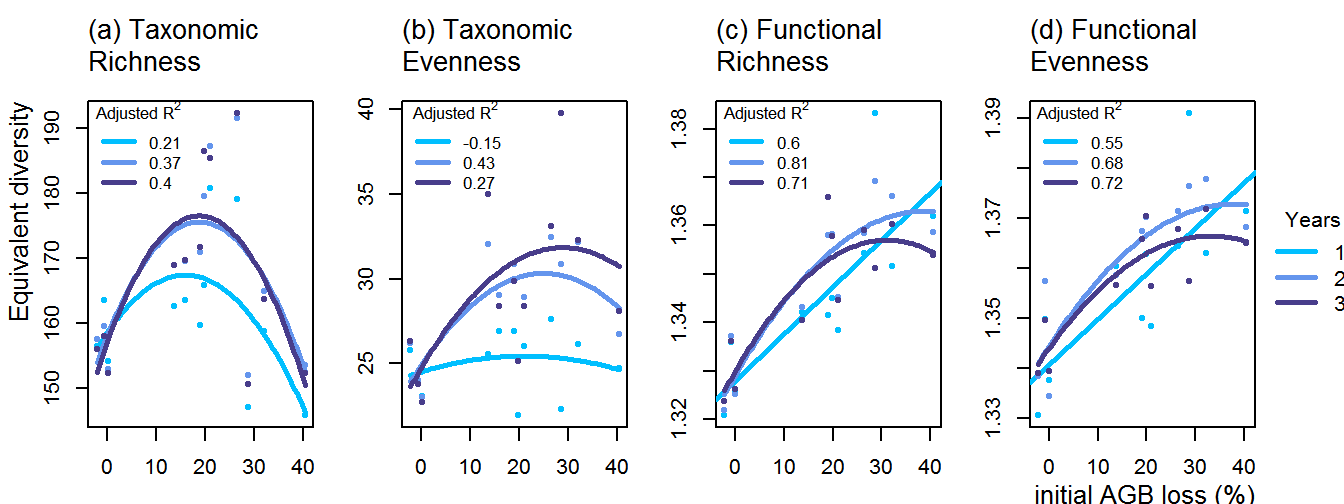
\includegraphics[width=1\linewidth]{WholePlotTrajectories_files/figure-latex/IDHplot-1} 

}

\caption{Upper panels, Trajectories of the Simpson taxonomic diversity \textbf{(a)} and Rao functional diversity \textbf{(b)} over 30 years after disturbance. Colors are treaments: green (control), blue (T1), orange (T2), red (T3) with sahded areas the credibility intervals. Lower panels, Relationship between the initial \%AGB removed and Simpson \textbf{(c)} and Rao \textbf{(d)} diversities, 10, 20 and 30 years after disturbance}\label{fig:IDHplot}
\end{figure*}

\subsection{Communities Composition}\label{communities-composition}

\subsubsection{Taxonomic and functional
trajectories}\label{taxonomic-and-functional-trajectories}

While both taxonomic and functional composition remained stable in
undisturbed communities (ref to fig), they followed consistent trajectories over time
after disturbance. According to the mapping of functional traits (see appendix I) these
compositional changes corresponded to shifts towards species with more
acquisitive functional strategies, from communities with high average WD
to high average SLA and chlorophyll content. For disturbed communities
the distance of successive inventories to the 1989 reference inventory
followed unimodal trajectories translating cyclic compositional changes
with a recovery of the initial composition (Figure \ref{fig:NMDSplans}).
The maximum dissimilarity with the initial state was positively
correlated to the disturbance treatment for both taxonomic and
functional composition (\(\rho_{spearman}^{taxonomic}=0.91\) and
\(\rho_{spearman}^{functional}=0.96\) respectively) and the time at
maximum was reached around 26 years after disturbance for taxonomic
composition and 22 years for functional composition.

\begin{figure*}

{\centering 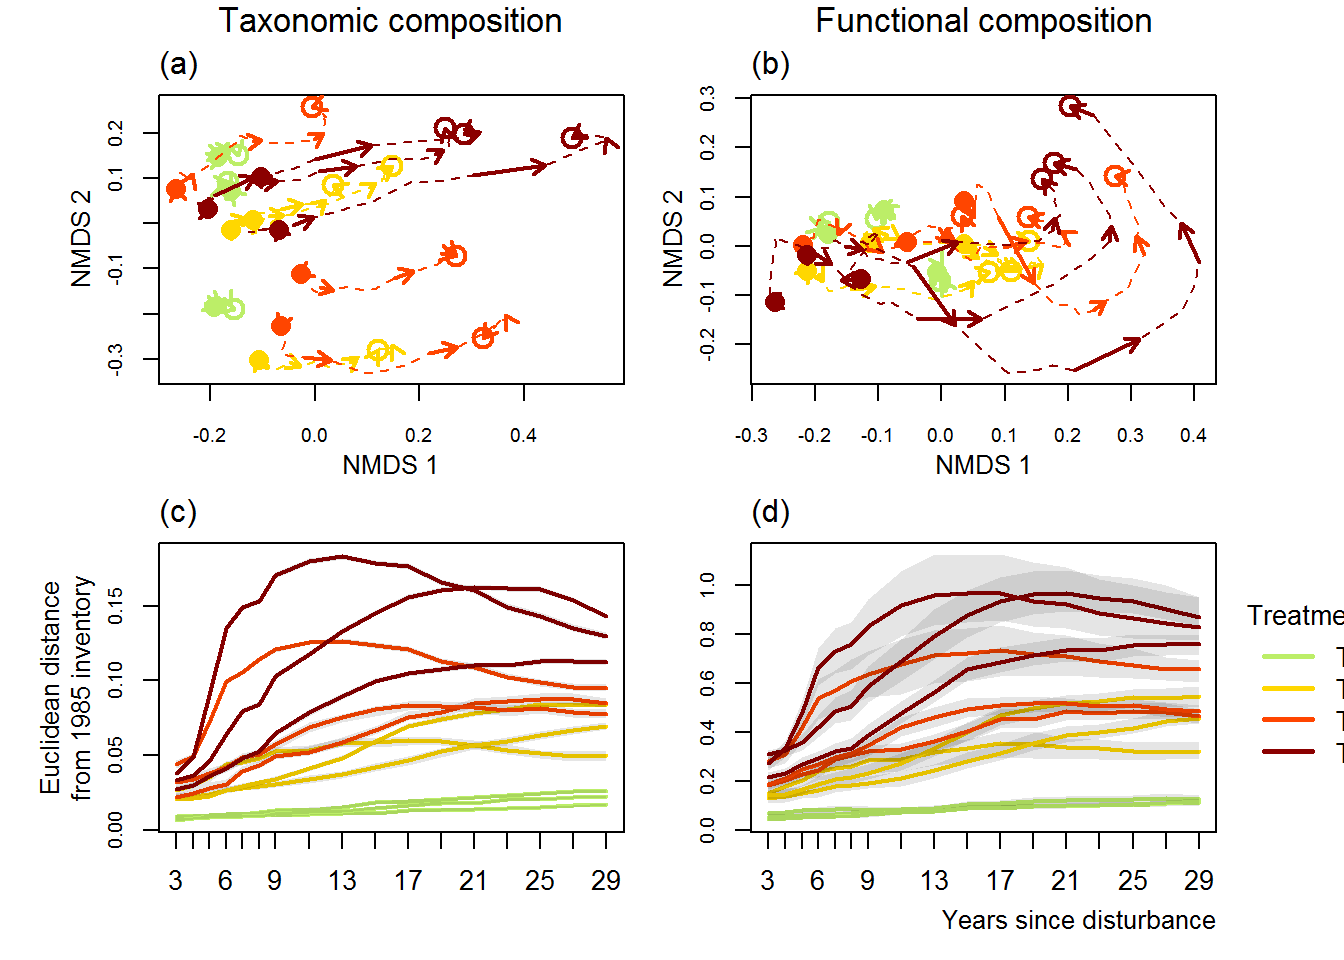
\includegraphics[width=1\linewidth]{WholePlotTrajectories_files/figure-latex/NMDSplans-1} 

}

\caption{Plot trajectories in terms of flora composition (left panels \textbf{(a)} and \textbf{(c)}) and functional composition (right panels \textbf{(b)} and \textbf{(d)}) in a the two-dimensional NMDS space. Lower panels (\textbf{(c)} and \textbf{(d)}) represent the euclidean distance to initial condition along the 30 sampled years. Colors are disturbance treatments (green for control, blue for T1,orange for T2 and red for T3) with shaded areas, the credibility intervals}\label{fig:NMDSplans}
\end{figure*}

\subsubsection{Traits community weighted means
(CWM)}\label{traits-community-weighted-means-cwm}

Changes in functional composition trajectories went hand to hand
with consistent trajectories of the 8 functional traits (Figure
\ref{fig:CWM}). Except for leaf chlorophyll content, which continued to increase for
some T3 and T2 plots 30 years after disturbance, all traits and seed
mass proportions followed unimodal trajectories either stabilizing or
returning towards their initial values. Thirty years after disturbance
the weighted means of communities specific maximum height at adult stage
(\emph{Hmax}), leaf toughness (\emph{L\_toughness}) and wood specific
gravity (\emph{WD}) remained significantly lower than their initial
value (Figure \ref{fig:CWM}). The weighted means of bark thickness
(\emph{Bark\_thick}) similarly remained substantially higher than
initially for all disturbed plots while the specfic leaf area
(\emph{SLA}) had almost recovered its initial value. For all traits the
maximum difference to initial state was correlated to the disturbance
intensity (\(\rho_{spearman}^{L_{thickness}}=0.67\),
\(\rho_{spearman}^{L_{chloro}}=0.45\),
\(\rho_{spearman}^{L_{toughness}}=-0.43\),
\(\rho_{spearman}^{SLA}=0.93\), \(\rho_{spearman}^{WD}=-0.78\),
\(\rho_{spearman}^{Bark-thickness}=0.88\),
\(\rho_{spearman}^{Hmax}=-0.48\)).

\begin{figure*}

{\centering 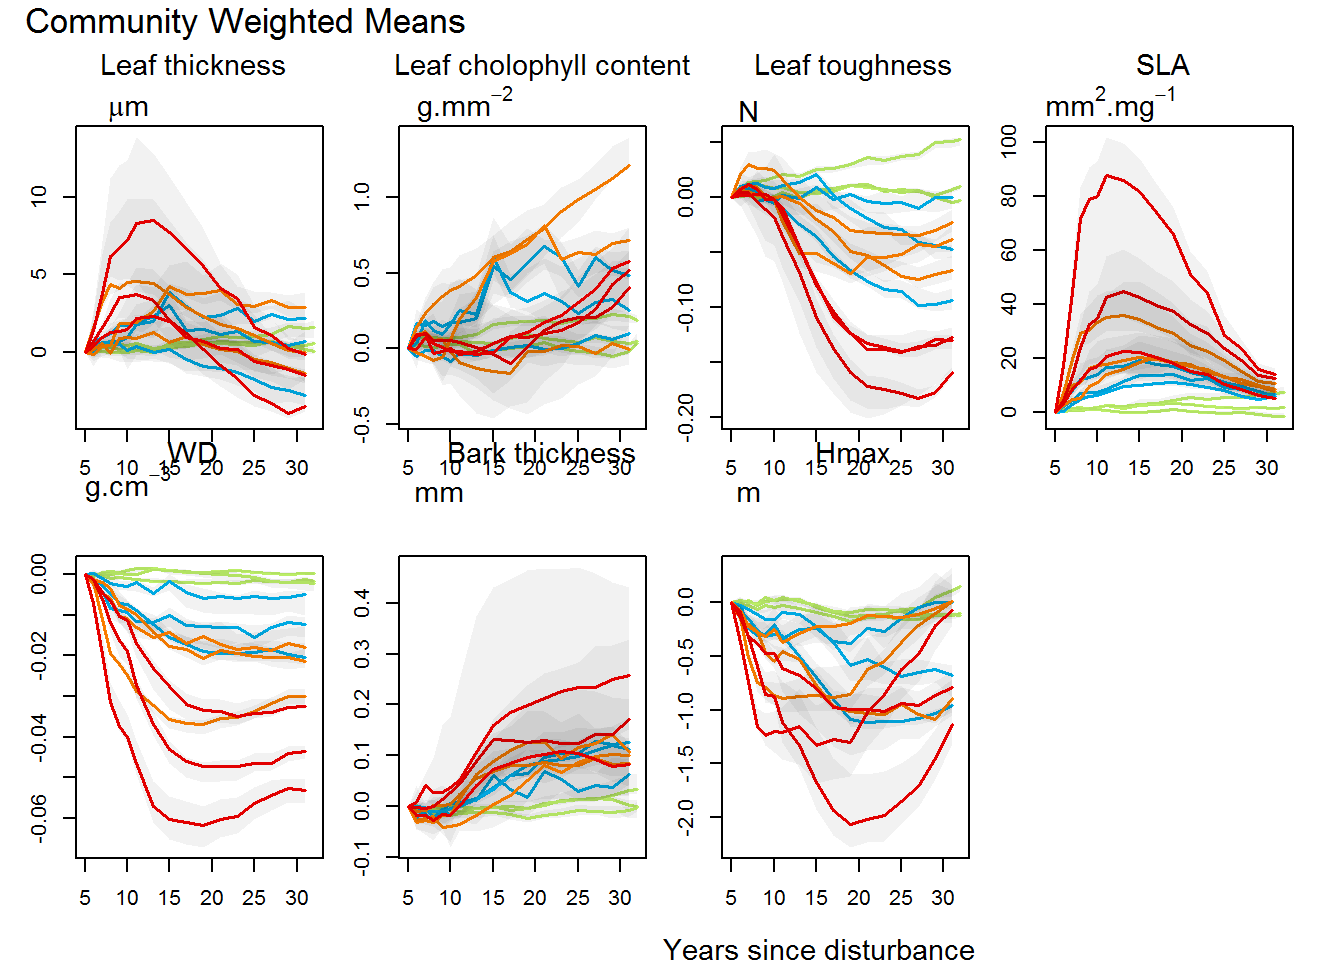
\includegraphics[width=1\linewidth]{WholePlotTrajectories_files/figure-latex/CWM-1} 

}

\caption{Trajectories of the communities weighted means (CWM) over 30 years after disturbance of 4 leaf traits (Leaf thickness, \emph{L\_thickness}, chlorophyll content, \emph{L\_chloro}, toughness, \emph{L\_toughness} and specific area, \emph{SLA}), 2 stem traits (wood specific gravity, \emph{WD}, and bark thickness, \emph{Bark-thick}) and one life history trait (Specific maximum height at adult stage, \emph{Hmax}). Colors are disturbance treatments: green (control), blue (T1), orange (T2), red (T3) with shaded areas the credibility intervals.}\label{fig:CWM}
\end{figure*}

\subsubsection{Functional redundancy}\label{functional-redundancy}

Communities functional redundancy remained stable in control
plots but after disturbance the redundancy trajectories were quite
variable (See appendix I) and apparently independently of the initial
disturbance. Globally after most intense disturbance (plots T2 and T3)
communities redundancy decreased at first place before increasing to
edge, recover or exceed the initial value. *I would suggest to consider only the Functional redundancy restricted to the functional space in the paper*

Considering the functional redundancy restricted to the functional space
of the initial inventory, all disturbed plots followed similar
decreasing humped shaped trajectories (@ref(fig:RedFun\_rest)). The
maximum redundancy loss was positively correlated with the disturbance
intensity (\(\rho_{spearman}=0.50\)) and the initial value had not
recovered for any disturbed communities.

\begin{figure}

{\centering 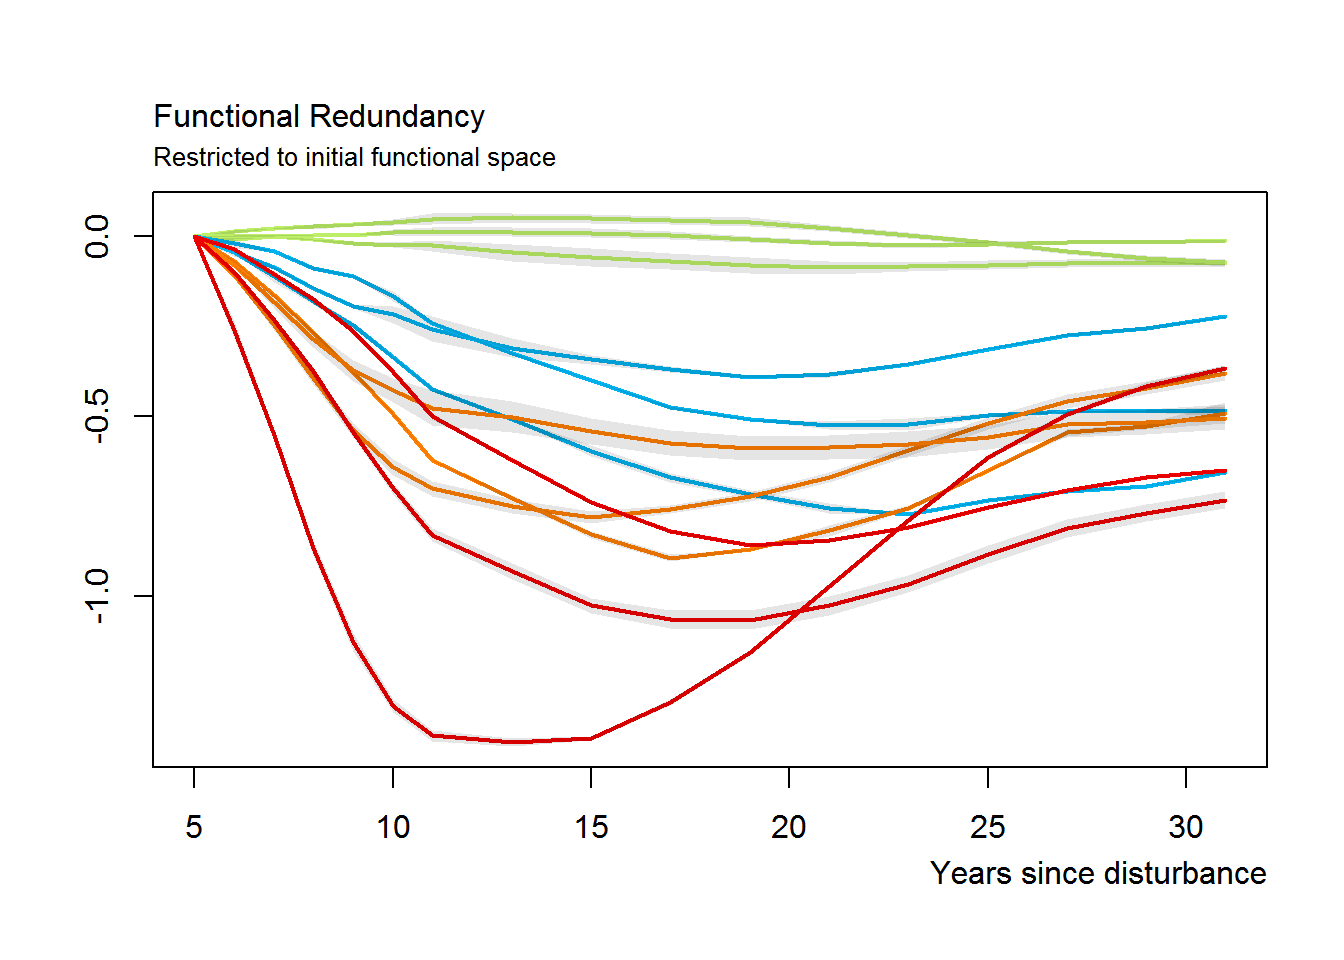
\includegraphics[width=1\linewidth]{WholePlotTrajectories_files/figure-latex/RedFun_rest-1} 

}

\caption{Trajectories of functional redundancy within the initial functional space over 30 years after disturbance. Colors are disturbance treatments: green (control), blue (T1), orange (T2), red (T3) with shaded areas the credibility intervals.}(\#fig:RedFun_rest)
\end{figure}

\section{Discussion}\label{discussion}

\subsection{Decoupled taxonomic and functional
trajectories}\label{decoupled-taxonomic-and-functional-trajectories}

Both communities taxonomic and functional diversities and composition
proved resilient, following similar humped shaped trajectories returning
towards initial values. Communities functional structure is the most
direct link between biodiversity and ecosystem functioning
\citep{Diaz2005} and its resilience meant the recovery of ecosystem
processes in the long term \citep{Guariguata2001}. The resilience of
communities taxonomy in turn meant the maintenance of their initial
differences in species composition and diversity. The maintenance of
initial differences suggested the existence of multiple stable
equilibria as assumed for highly diverse and productive ecosystems
\citep{Chase2003} and the dependency of recovery trajectories on the
initial composition to be recovered
\citep{Hubbell1999, Molino2001, Anderson2007, Baraloto2012a}.

Although communities taxonomic and functional trajectories were similar
the taxonomic recovery lagged behind the functional one, confirming a
decoupling between functional and taxonomic dynamics already observed
for grasslands \citep{Tilman1997, Mouillot2011} and tropical forests
\citep{Lohbeck2015, Guariguata2001}. According to the ``vegetation
quantity effect'' \citep{Grime1998} the functional trajectories rely on
the pool of dominant species, which diversity and evenness increased and
rapidly recovered after disturbance. At the same time communities
taxonomic evenness remained high, revealing the unachieved recovery of
infrequent species.

\subsection{The extent of the intermediate disturbance
hypothesis}\label{the-extent-of-the-intermediate-disturbance-hypothesis}

The taxonomic and functional trajectories validated the IDH as
determinant of communities functional structure and of the dominant
species pool, while contrastingly the pool of rare species relied upon
more stochastic processes.

The disturbance intensity poorly predicted the taxonomic richness, as
already observed in the Paracou station \citep{Baraloto2012a} and in
Bornean tropical forests \citep{Cannon1998}, was only weakly correlated
with the increase in taxonomic evenness (\emph{i.e.} Simpson diversity).

Contrastingly, the disturbance intensity consistently predicted the
increase in functional diversity after disturbance along the 30 years.
The functional diversity increase paralleled the significant specific
turnover and functional shifts towards resource-acquisitive strategies
(sharp increase in the SLA, leaf thickness and bark thickness and
decrease in wood density, leaf toughness and maximum height)
\citep{Westoby1998, Wright2004, Reich2014}. As the old-growth,
pre-disturbance survivor trees proved mirroring the initial communities
\citep{Herault2018} the functional trajectories and taxonomic turnover
rather relied upon the pool of newly recruited trees driven by the
enhanced growth and survival of previously infrequent species and
functional types. Disturbance entailed a reorganization, benefiting to
pioneers and light demanding species, of the typical high dominance
structure of hyperdiverse mature forests. The changes in abiotic
environment and competitive pressure favored pioneers which outcompeted
other species in non limiting light resources but were excluded in
mature forests by long-lived, more resistant and shade tolerant species.
Disturbance trajectories therefore relied upon the environmental niches
made available and filled by species from a restricted functional range
that became dominant and structured the functional characteristics of
the community \citep{Grime1998}. The intermediate disturbance hypothesis
was suitabe to predict communities functional diversity and pool of
dominant species \citep{Molino2001}, but it poorly represented the whole
taxonomic structure that was hampered by the slow recovery of rare
species \citep{Hubbell2001, Chave2004}.

\subsection{The functional redundancy, key of communities
resilience}\label{the-functional-redundancy-key-of-communities-resilience}

The functional and taxonomic decoupling and the rebuttal of the IDH for
communities taxonomic structure were explained by a reorganization of
the functional redundancy within the functional traits space that
implied the incomplete resilience of communities
\citep{Trenbath1999, Elmqvist2003, Diaz2005}.

Although the functional redundancy considered in the functional space of
the whole communities did not display consistent trajectories after
disturbance, the redundancy restricted to the functional space of the
initial community clearly followed humped shaped trajectories. After
disturbance communities differently occupied the functional space,
following the observed shifts in traits trajectories and functional
composition, and the redundancy in the initial functional space
decreased according to the disturbance intensity. After 30 years the
recovery of the initial redundancy structure was consistent but remained
unachieved. It depended on infrequent species specific to old-growth
forests that were functionally and therefore underwent competitive
exclusion limiting functional similarity
\citep{Chave2004, Mayfield2010}. The persistent alteration of functional
redundancy meant a lower resilience of pre-disturbance communities and
an higher resilience disturbance-specific communities (corresponding to
lower richness and higher dominance of pioneer species) so chances to
observe self-maintained compositional changes in favor of disturbance
resistant species, lianas or epiphytes were increased after disturbance
\citep{Haddad2008, Burslem2000, Martin2013}. Communities resilience
depended on the functional redundancy structure that proved long to
recover. This decades-long recovery specifically increased the risks of
loosing cornerstone specie, with unexpected ecological consequences
\citep{Jones1994, Chazdon2003a, Diaz2005, Gardner2007}.

\section{Conclusions}\label{conclusions}

Our study defined the decoupled functional and taxonomic trajectories of
tropical rainforests after disturbance demonstrating a rapid functional
recovery but a slower and more variable taxonomic one. Consistently with
the IDH, functional trajectories were driven after disturbance by
deterministic processes favoring pioneers and light-demanding species.
The following functional shifts entailed a re-organization of
communities functional redundancy that proved long to recover and
explained the more variable and longer taxonomic trajectories as shade
tolerant species of old-growth forests faced functional redundancy and
limiting similarity processes. The resilience of tropical forests then
proved long in the face of quite intense disturbance and did not
preclude the settling of a persistent disturbance-specific community
\citep{Gourlet-Fleury2005}. As the trajectories highlighted the
recruitment processes proved central for communities response to
disturbance and closer focus on demographical drivers of communities
response would clarify the fate of the future forests. The disturbance
range however stayed within the spectrum of selective logging, with a
forest cover remaining all along the experiment, and the response
mechanisms would probably be much different after harder disturbance.

%----------------------------------------------------------------------------------------
%	REFERENCE LIST
%----------------------------------------------------------------------------------------

\bibliographystyle{mee}
\makeatletter
% The filename has .bib extension the must be eliminated
\filename@parse{references.bib}
% parse stores the file name in base. Extension starts at the first dot, so don't use dots in file names.
\bibliography{\filename@base}
\makeatother


%----------------------------------------------------------------------------------------

\end{document}
